\documentclass{beamer}

\usepackage{beamerthemesplit}
\usepackage[utf8]{inputenc}
% \usepackage[danish]{babel}
\usepackage[T1]{fontenc}
\usepackage{graphicx}
\usepackage{amsmath}
\usepackage{hyperref}
\usepackage{enumerate}
\usepackage{url}


\title{2. Seminar EVU RegAut}
\author{Sigurd Meldgaard}
\date{26. January 2009}

\AtBeginSection[]
{
   \begin{frame}
       \frametitle{Plan}
       \tableofcontents[currentsection]
   \end{frame}
}

\begin{document}
\maketitle

%\section{Nondeterministiske automater}
\begin{frame}
\frametitle{Ækvivalens ml. Regulære udtryk og FA'er}
  \begin{itemize}[<+->]
  \item Definition af NFA’er og deres sprog
\item Delmængdekonstruktionen:  NFA $\rightarrow$ FA
\item Definition af NFA-$\Lambda$’er og deres sprog
\item $\Lambda$-eliminering:  NFA-$\Lambda$ $\rightarrow$ FA
\item Kleenes sætning: regulært udtryk $\rightarrow$ NFA-$\Lambda$ $\rightarrow$ NFA $\rightarrow$ FA $\rightarrow$ regulært udtryk
  \end{itemize}
\end{frame}


\begin{frame}
\frametitle{Nondeterministiske automater}
\begin{itemize}[<+->]
\item  NFA’er: som FA’er men
\item Der er ikke altid præcis én udgående transition pr. alfabetsymbol for hver tilstand
\item Automaten accepterer en streng, hvis det er muligt at ``gætte'' en vej til accept
\end{itemize}

\end{frame}

\begin{frame}
\frametitle{Eksempel}

\begin{columns}
  \begin{column}{9cm}
    \begin{itemize}[<+->]
    \item Hvordan laver man en automat, der svarer til det regulære
      udtryk $(11 + 110)^*0$ ?

    \item Det er ikke trivielt med FA’er...

    \item En nondeterministisk automat:
    \end{itemize}
  \end{column}
  \begin{column}{5cm}
\visible<3->{
      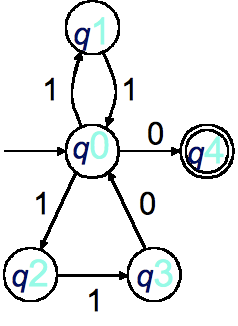
\includegraphics[scale=0.4]{images/2_seminar_quiz_NFA}}
  \end{column}
\end{columns}
\end{frame}
\begin{frame}
\frametitle{Formel definition af NFA}
\begin{verse}
Everything is vague to a degree you do not realize till you have tried to make it precise.
\end{verse}
    Bertrand Russell

    \bigskip  

\pause
En nondeterministisk endelig automat (NFA) er et 5-tupel $(Q, \Sigma, q_0, A, \delta)$ hvor
 
\begin{itemize}[<+->]
\item $Q$ er en endelig mængde af tilstande
\item $\Sigma$ er et alfabet
\item $q_0\in Q$ er en starttilstand
\item $A\subseteq Q$ er accepttilstande
\item $\delta$: $Q\times \Sigma \rightarrow$ \alert{$2^Q$} er en transitionsfunktion\\
  Det betyder at $\delta(q,a)$ giver en \emph{mængde} af tilstande.
\end{itemize}
\end{frame}

\newcommand{\sarrow}[1]{\overset{#1}{\rightarrow}}

\begin{frame}
\frametitle{Eksempel på en NFA}
\begin{columns}
\column{9cm}Her er den grafiske representation af en automat:
\column{3cm}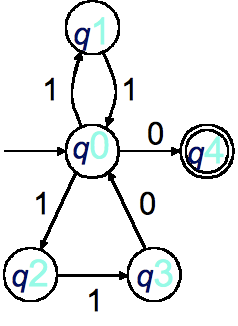
\includegraphics[scale=0.3]{images/2_seminar_quiz_NFA}
\end{columns}
\begin{itemize}[<+->]
  \item Den representerer 5-tuplet:
  \item $Q=\{q_0,q_1,q_2,q_3,q_4\}$
  \item $\Sigma = \{0,1\}$
  \item $A=\{q_4\}$
  \item
      $\delta$ : $Q\times \Sigma \rightarrow 2^Q$ Er funktionen i
      denne tabel: \scalebox{0.7}{
        \begin{tabular}{|l|ll|}
          \hline
          & 0 & 1 \\
          \hline
          $q_0$ & $\{q_4\}$ & $\{q_1, q_2\}$ \\
          \hline
          $q_1$ & $\emptyset$ & $\{q_0\}$ \\
          \hline
          $q_2$ & $\emptyset$ & $\{q_3\}$ \\
          \hline
          $q_3$ & $\{q_0\}$ & $\emptyset$ \\
          \hline
          $q_4$ & $\emptyset$ & $\emptyset$ \\
          \hline
        \end{tabular}}

  \end{itemize}
\end{frame}
\begin{frame}
\frametitle{Sproget af en NFA}
Givet en NFA $M=(Q, \Sigma, q_0, A, \delta)$:
\begin{itemize}[<+->]
\item Definer den udvidede transitionsfunktion:
\[\delta^*(q, x) = \begin{cases}
  \{q\} & \text{ hvis } x=\Lambda \\
  \bigcup_{r\in \delta^*(q,y)}\delta(r, a)& \text{ hvis } x=y\cdot a
\end{cases}
\]
\item $x\in \Sigma^*$ accepteres af en NFA $M$ hvis og kun hvis $\delta^*(q_0,x) \cap A \neq \emptyset$
\item $L(M)=\{x | x \text{ accepteres af } M\}$
\end{itemize}
\end{frame}
\begin{frame}
\frametitle{NFA'er er ofte mindre end FA'er}
\begin{itemize}[<+->]
\item $L_{42}=\{x \mid |x|\geq 42 \wedge \text{ 42 tegn fra højre er et 1} \}$
\item Sidste seminar viste vi at det kræver mindst $2^{42}$ tilstande
  at lave en FA der genkender $L_{42}$
\item En \alert{N}FA der genkender $L_{42}$ med 43 tilstande:
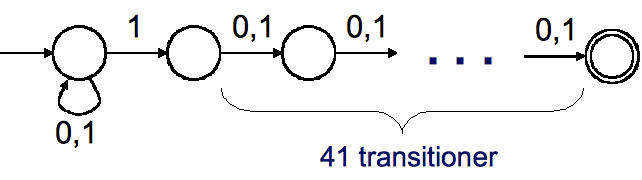
\includegraphics[scale=0.4]{images/2_seminar_L42_NFA}
\end{itemize}
\end{frame}
\begin{frame}
\frametitle{Quiz}
\begin{columns}
\column{5cm} Bliver strengen 110110 accepteret af denne automat?
\column{5cm}
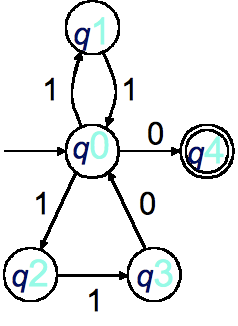
\includegraphics[scale=0.4]{images/2_seminar_quiz_NFA}
\end{columns}
\visible<2->{
Ja! der findes en sti til accept:
\[
q_0 \sarrow{1} q_2 \sarrow{1} q_3 \sarrow{0} q_0 \sarrow{1} q_1 \sarrow{1} q_0 \sarrow{0} q_4 
\]}
\visible<3->{Vi kan systematisk lede efter sådan en sti: $\{q_0\} $}
$
\visible<4->{\sarrow{1} \{q_1, q_2\}}
\visible<5->{\sarrow{1} \{q_0, q_3\}} $
$\visible<6->{\sarrow{0} \{q_4, q_0\} \sarrow{1} \{q_1, q_2\} \sarrow{1} \{q_0, q_3\} \sarrow{0} 
\{q_4, q_0\}}$
\end{frame}
\begin{frame}
\frametitle{Øvelser:}
\begin{itemize}
\item{} [Martin]: opg. 4.2. (p. 156)
Drawing an NFA and using the definition of $\delta^*$
\end{itemize}
\end{frame}

\section{Determinisering}
\begin{frame}
\frametitle{Enhver FA kan oversættes til en NFA}
\begin{itemize}[<+->]
\item Hvis man ser på den grafiske repræsentation, så er det trivielt,
  en FA er bare en simpel NFA.
\item Formelt: givet en FA: $N=(Q, \Sigma, q_0, A, \delta)$
\item Konstruer en NFA: $M=(Q, \Sigma, q_0, A, \delta')$ hvor:
  
\[\delta'(q,a) = \{\delta(q,a)\}\]
\item Husk bevis for korrekthed! $L(M)=L(N)$ fordi... (induktion i længden af en inputstreng)
\end{itemize}
\end{frame}

\begin{frame}
\frametitle{Enhver NFA kan oversættes til en FA}
\begin{center}
  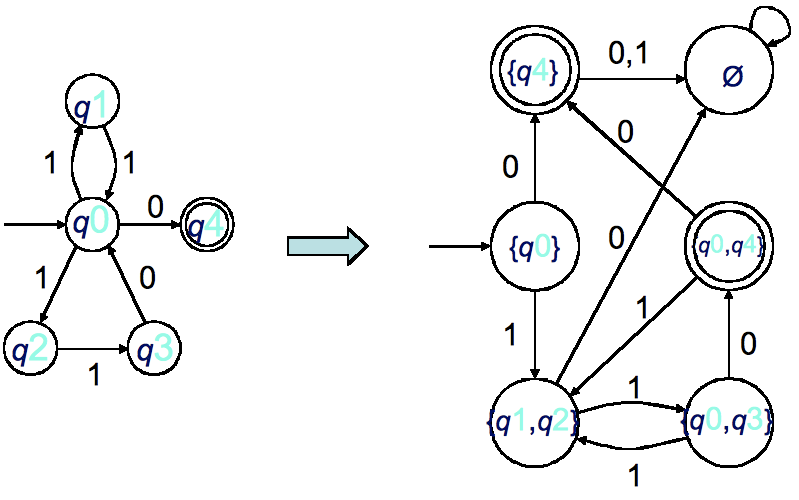
\includegraphics[scale=0.3]{images/2_seminar_convert}
\end{center}
\pause

Dette kaldes determinisering
\end{frame}

\begin{frame}
\frametitle{Delmængdekonstruktionen (determinisering)}
Givet en NFA: $N=(Q, \Sigma, q_0, A, \delta)$

Konstruer en FA: $M=(Q', \Sigma, q_0', A', \delta')$
\pause
\begin{itemize}[<+->]
\item $Q'=\alert{2^{Q}}$ (tilstandene i FA'en svarer til en mængde af tilstande i NFA'en)
\item $q_0' = \{q_0\}$
\item $A' = \{q \in Q' | A \cap q \neq \emptyset \}$
\item $\delta'(q, a) = \bigcup_{r\in q}\delta(r,a)$
\item Husk bevis for korrekthed...
\end{itemize}
\end{frame}
\begin{frame}
  \frametitle{Bevis for korrekthed af delmængdekonstruktionen}
\begin{itemize}[<+->]
\item Husk definitionen for $L(M)$ og $L(N)$
\[L(M) = \{x | \delta'^*(q_0', x) \in A'\}\]
\[L(N) = \{x | \delta^*(q_0, x) \cap A \neq \emptyset\}\]
\item Lemma:
\[\forall x\in \Sigma^*: \delta'^*(q_0', x) = \delta^*(q_0, x)\]
Bevis: induktion i strukturen af $x$...
\item $ \delta'^*(q_0', x) \in A' \overset{\text{\tiny{lemma}}}{\Leftrightarrow} 
 \delta^*(q_0, x) \in A' \overset{\text{\tiny{def af A}}}{\Leftrightarrow} \delta^*(q_0, x) \cap A \neq \emptyset$
\item D.v.s. $L(M)=L(N)$
\end{itemize}
\end{frame}

\begin{frame}
\frametitle{Nøjes med opnåelige tilstande}
\begin{itemize}[<+->]
\item Delmængdekonstruktionen bruger $Q' = 2^Q$
\item Som ved produktkonstruktionen: I praksis er hele tilstandsrummet
  sjældent nødvendigt
\item Som sidste gang: Kun tilstande, der er opnåelige fra
  starttilstanden er relevante for sproget (Bevis dette: Opg. 3.29, p. 117)
\end{itemize}
\end{frame}
\begin{frame}
\frametitle{Øvelser}
\begin{itemize}
\item{} [Martin] Opg. 4.10 (a+e) (p. 157)\\
Udfør selv delmængdekonstruktionen.
\end{itemize}
\end{frame}

\section{NFA-$\Lambda$’er}
\begin{frame}
  \frametitle{NFA'er med $\Lambda$-transitioner}
\begin{itemize}[<+->]
\item For nemt at kunne oversætte regulære udtryk til automater
  generaliserer vi automaterne yderligere
\item En $\Lambda$-transition er en transition, der ikke læser et
  symbol fra input-strengen
\item Eksempel på en NFA-$\Lambda$:
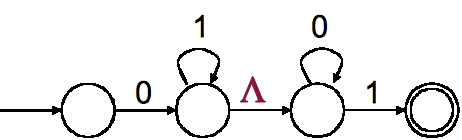
\includegraphics[scale=0.4]{images/2_seminar_nfalambda}
\item Automaten “bestemmer selv” om den vil følge 
$\Lambda$-transitionen
Eksempel: strengen 011 accepteres
\end{itemize}
\end{frame}
\begin{frame}
\frametitle{Formel definition af NFA-$\Lambda$}
En nondeterministisk endelig automat 
med $\Lambda$-transitioner (NFA-$\Lambda$) er 
et 5-tupel $(Q, \Sigma, q_0, A, \delta)$ hvor

\begin{itemize}[<+->]
\item $Q$ er en endelig mængde af tilstande
\item $\Sigma$ er et alfabet
\item $q_0\in Q$ er en starttilstand
\item $A\subseteq Q$ er accepttilstande
\item $\delta: Q\times (\Sigma \alert{\cup \{\Lambda}\})\rightarrow 2^Q$ er en
  transitionsfunktion
\end{itemize}
\end{frame}
\begin{frame}
\frametitle{$\Lambda$-lukning af en tilstandsmængde ($\Lambda$-closure)}
\begin{itemize}[<+->]
\item Hvor kan man komme til ved kun at bruge 
$\Lambda$-transitioner?
\item Givet en mængde $S\subseteq Q$, definer $\Lambda$-lukningen
  $\Lambda(S)$ som den mindste mængde der opfylder flg.: 
\item $S \subseteq \Lambda(S)$
\item $\forall q\in \Lambda(S): \delta(q, \Lambda) \in \Lambda(S)$
\end{itemize}
\end{frame}

\begin{frame}
\frametitle{Sproget for en NFA-$\Lambda$}
\begin{itemize}[<+->]
\item Givet en NFA-$\Lambda$  $M=(Q, \Sigma , q_0, A, \delta )$, definer 
den udvidede transitionsfunktion $\delta^*: Q\times \Sigma^*\rightarrow  2^Q$ ved
\item \[\delta^*(q,x) =
  \begin{cases}
    \Lambda(q) & \text{ hvis } x=\Lambda \\
    \Lambda(\bigcup_{r\in \delta^*(q, y)}\delta(r, a)) & \text{ hvis } x=y\cdot a
  \end{cases}
\]
\item $L(M) = \{x \in \Sigma^* | \delta^*(q_0, x)\cap A \neq \emptyset \}$
\end{itemize}
\end{frame}
\begin{frame}
\frametitle{Quiz}
\begin{itemize}[<+->]
\item Hvad er $\delta^*(q_0, 01)$ for denne NFA-$\Lambda$?
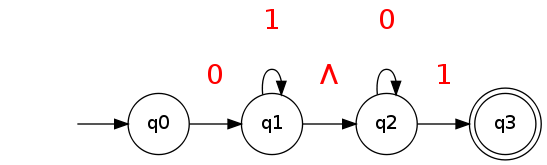
\includegraphics[scale=0.4]{images/2_seminar_quiz_nfa_lambda}
\item $\delta^*(q_0, \Lambda) = \Lambda(q_0) = \{q_0\}$
\item $\delta^*(q_0, \Lambda \cdot 0) = \Lambda(\bigcup_{r\in \delta^*(q_0, \Lambda)} \delta(r, 0)) =
 \{q_1, q_2\}$
\item $\delta^*(q_0, \Lambda \cdot 0 \cdot 1) = 
\Lambda(\bigcup_{r\in \delta^*(q_0, \Lambda\cdot 0)} \delta(r, 1)) = \Lambda(\{q_1, q_2\}\cup\{q_3\}) = \{q_1, q_2, q_3\}$
\item - d.v.s. strengen 01 bliver accepteret af automaten.
\end{itemize}
\end{frame}

\begin{frame}
  \frametitle{Enhver NFA kan oversættes til en NFA-$\Lambda $}
\begin{itemize}[<+->]
\item Med den grafiske repræsentation er det trivielt

\item Med de formelle definitioner:

Givet en NFA $M=(Q, \Sigma , q_0, A, \delta_M)$, 

definer en NFA-$\Lambda $ $N=(Q, \Sigma , q_0, A, \delta_N)$ hvor 
$\delta_N(q, a) = \delta M(q, a)$  for alle $q\in Q$ og $a\in \Sigma$
$\delta_N(q, \Lambda) = Ø$ for alle $q\in Q$

Bevis for at $L(N) = L(M)$: induktion...
\end{itemize}
\end{frame}

\begin{frame}
\frametitle{Enhver NFA-$\Lambda $ kan oversættes til en NFA
($\Lambda $-eliminering)}
\begin{itemize}[<+->]
\item Givet en NFA-$\Lambda $ $M=(Q, \Sigma , q_0, A, \delta )$, 
\item definer en NFA $M_1=(Q, \Sigma , q_0, A_1, \delta _1)$ ved
\item $\delta _1(q, a) =  \delta ^*(q, a)$
\item $A_1 =
  \begin{cases}
    A \cup \{ q_0\} & \text{ hvis } \Lambda(\{q_0\})\cap A \neq \emptyset \\
    A & \text{ ellers }
  \end{cases}
$
\item Der gælder nu: $L(M_1) = L(M)$
\end{itemize}
\end{frame}

\begin{frame}
\frametitle{Eksempel}
\begin{itemize}[<+->]
\item NFA-$\Lambda$:
\begin{center}
  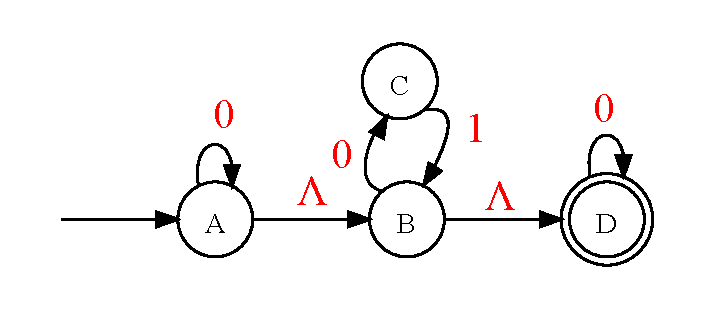
\includegraphics[scale=0.4]{images/2_seminar_lambdaelim}
\end{center}
\item Find $\delta^*(q,a)$ for alle $q\in Q$ og $a\in \Sigma$
\item Se om $\Lambda(\{q_0\})\cap A \neq \emptyset$
\end{itemize}

\begin{columns}
\column{5cm}
\scalebox{0.6}{
  \begin{tabular}{|c|ccc|cc|}
    \hline
    $q$ & $\delta(q,\Lambda)$ & $\delta(q, 0)$ & $\delta(q, 1)$ & $\delta^*(q,0)$ & $\delta^*(q,1)$\\
    \hline
    A & $\{B\}$ & $\{A\}$ & $\{\}$ & \{A,B,C,D\} & \{\} \\
    B & $\{D\}$ & $\{C\}$ & $\{\}$ & \{C,D\} & \{\} \\
    C & $\{\}$ & $\{\}$ & $\{B\}$ & \{\} & \{B,D\} \\
    D & $\{\}$ & $\{D\}$ & $\{\}$ & \{D\} & \{\} \\
    \hline
  \end{tabular}
  }
\column{5cm}
  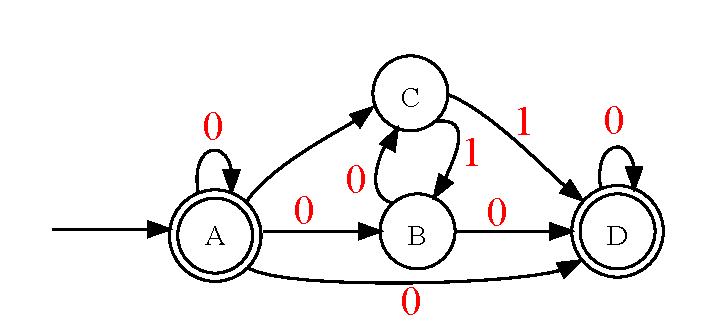
\includegraphics[scale=0.4]{images/2_seminar_lambdaelim2}
\end{columns}
\end{frame}

\begin{frame}
\frametitle{Bevis for korrekthed af $\Lambda $-eliminering}
\begin{itemize}[<+->]
\item Vi skal vise:  $\forall x\in \Sigma^*: x \in L(M_1) \Leftrightarrow x\in L(M)$
$x=\Lambda$ : brug definition af $A_1$ og $\Lambda$-lukning...
\item $x=a \in \Sigma$ : brug $A_1$, $\delta^*(q,a)=\delta_1(q,a)$ og $\Lambda$-lukning...
\item
$x = ya, y\neq \Lambda$:
Induktionshypotese:  $\forall y\in \Sigma^*, y\neq \Lambda :  \delta^*(q_0, y) = \delta_1(q_0, y)
\Rightarrow \delta^*(q_0, x) = \delta_1^*(q_0, x)$

...

\item
– se bogen Th. 4.2 p. 141.
\end{itemize}
\end{frame}
\begin{frame}
\frametitle{Øvelser}
\begin{itemize}
\item{} [Martin] Opg. 4.13 (p.159)
Kør strenge på en NFA-$\Lambda$
\item{} [Martin] Opg. 4.28 (e)
Brug algoritmen til $\Lambda$-eliminering
\end{itemize}
\end{frame}


%%% Local Variables: 
%%% mode: latex
%%% TeX-master: "2_seminar"
%%% End: 

\section{NFA-$\Lambda$’er}
\begin{frame}
  \frametitle{NFA'er med $\Lambda$-transitioner}
\begin{itemize}[<+->]
\item For nemt at kunne oversætte regulære udtryk til automater
  generaliserer vi automaterne yderligere
\item En $\Lambda$-transition er en transition, der ikke læser et
  symbol fra input-strengen
\item Eksempel på en NFA-$\Lambda$:
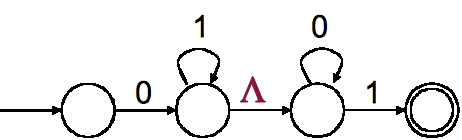
\includegraphics[scale=0.4]{images/2_seminar_nfalambda}
\item Automaten “bestemmer selv” om den vil følge 
$\Lambda$-transitionen
Eksempel: strengen 011 accepteres
\end{itemize}
\end{frame}
\begin{frame}
\frametitle{Formel definition af NFA-$\Lambda$}
En nondeterministisk endelig automat 
med $\Lambda$-transitioner (NFA-$\Lambda$) er 
et 5-tupel $(Q, \Sigma, q_0, A, \delta)$ hvor

\begin{itemize}[<+->]
\item $Q$ er en endelig mængde af tilstande
\item $\Sigma$ er et alfabet
\item $q_0\in Q$ er en starttilstand
\item $A\subseteq Q$ er accepttilstande
\item $\delta: Q\times (\Sigma \cup {\Lambda})\rightarrow 2^Q$ er en
  transitionsfunktion
\end{itemize}
\end{frame}

\begin{frame}
\frametitle{$\Lambda$-lukning af en tilstandsmængde ($\Lambda$-closure}
\begin{itemize}[<+->]
\item Hvor kan man komme til ved kun at bruge 
$\Lambda$-transitioner?
\item Givet en mængde $S\subseteq Q$, definer $\Lambda$-lukningen
  $\Lambda(S)$ som den mindste mængde der opfylder flg.: 
\item $S \in \Lambda(S)$
\item $\forall q\in \Lambda(S): \delta(q, \Lambda) \in \Lambda(S)$
\end{itemize}
\end{frame}

\begin{frame}
\frametitle{Sproget for en NFA-$\Lambda$}
\begin{itemize}[<+->]
\item Givet en NFA-$\Lambda$  $M=(Q, \Sigma , q_0, A, \delta )$, definer 
den udvidede transitionsfunktion $\delta^*: Q\times \Sigma^*\rightarrow  2^Q$ ved
\item \[\delta^*(q,x) =
  \begin{cases}
    \Lambda(q) & \text{ hvis } x=\Lambda \\
    \Lambda(\bigcup_{r\in \delta^*(q, y)}\delta(r, a)) & \text{ hvis } x=y\cdot a
  \end{cases}
\]
\end{itemize}
\end{frame}
\begin{frame}
\frametitle{Quiz}
\begin{itemize}[<+->]
\item Hvad er $\delta^*(q_0, 01)$ for denne NFA-$\Lambda$?
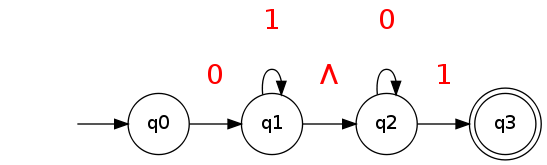
\includegraphics[scale=0.4]{images/2_seminar_quiz_nfa_lambda}
\item $\delta^*(q_0, \Lambda) = \Lambda(q_0) = \{q_0\}$
\item $\delta^*(q_0, \Lambda \cdot 0) = \Lambda(\bigcup_{r\in \delta^*(q_0, \Lambda)} \delta(r, 0)) =
 \{q_1, q_2\}$
\item $\delta^*(q_0, \Lambda \cdot 0 \cdot 1) = 
\Lambda(\bigcup_{r\in \delta^*(q_0, \Lambda\cdot 0)} \delta(r, 1)) = \Lambda(\{q_1, q_2\}\cup\{q_3\}) = \{q_1, q_2, q_3\}$
\item - d.v.s. strengen 01 bliver accepteret af automaten.
\end{itemize}
\end{frame}

\begin{frame}
  \frametitle{Enhver NFA kan oversættes til en NFA-$\Lambda $}
\begin{itemize}[<+->]
\item Med den grafiske repræsentation er det trivielt

\item Med de formelle definitioner:

Givet en NFA $M=(Q, \Sigma , q_0, A, \delta_M)$, 

definer en NFA-$\Lambda $ $N=(Q, \Sigma , q_0, A, \delta_N)$ hvor 
$\delta_N(q, a) = \delta M(q, a)$  for alle $q\in Q$ og $a\in \Sigma$
$\delta_N(q, \Lambda) = Ø$ for alle $q\in Q$

Bevis for at $L(N) = L(M)$: induktion...
\end{itemize}
\end{frame}

\begin{frame}
\frametitle{Enhver NFA-$\Lambda $ kan oversættes til en NFA
($\Lambda $-eliminering)}
\begin{itemize}[<+->]
\item Givet en NFA-$\Lambda $ $M=(Q, \Sigma , q_0, A, \delta )$, 
\item definer en NFA $M_1=(Q, \Sigma , q_0, A_1, \delta _1)$ ved
\item $\delta _1(q, a) =  \delta ^*(q, a)$
\item $A_1 =
  \begin{cases}
    A \cup \{ q_0\} & \text{ hvis } \Lambda(\{q_0\})\cap A \neq \emptyset \\
    A & \text{ ellers }
  \end{cases}
$
\item Der gælder nu: $L(M1) = L(M)$
\end{itemize}
\end{frame}
\begin{frame}
\frametitle{Eksempel}
\begin{itemize}[<+->]
\item NFA-$\Lambda$:
  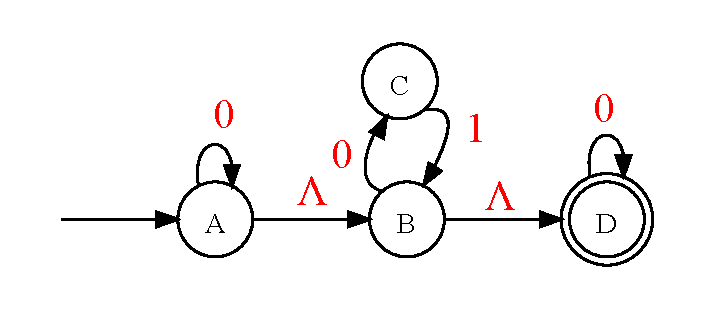
\includegraphics[scale=0.4]{images/2_seminar_lambdaelim}
\item Find $\delta^*(q,a)$ for alle $q\in Q$ og $a\in \Sigma$
\item Se om $\Lambda(\{q_0\})\cap A \neq \emptyset$
\item
  \begin{tabular}{|c|ccc|cc|}
    \hline
    $q$ & $\delta(q,\Lambda)$ & $\delta(q, 0)$ & $\delta(q, 1)$ & $\delta^*(q,0)$ & $\delta^*(q,1)$\\
    \hline
    A & $\{B\}$ & $\{A\}$ & $\{\}$ & \{A,B,C,D\} & \{\} \\
    B & $\{D\}$ & $\{C\}$ & $\{\}$ & \{C,D\} & \{\} \\
    C & $\{\}$ & $\{\}$ & $\{B\}$ & \{\} & \{B,D\} \\
    D & $\{\}$ & $\{D\}$ & $\{\}$ & \{D\} & \{\} \\

    \hline
  \end{tabular}

\end{itemize}
\end{frame}
\section{Kleenes sætning}
\section{Frokost}
\section{Minimering}
\section{Java projekt}
\end{document}